% !TeX root = ../presentation.tex

\setFooterToSchramm

{
    \metroset{sectionpage=none}
    \section{Einleitung}
}

\begin{frame}{Einleitung \footnotesize\cite{coppTrumpOfficialsTexted2025}}
    \begin{columns}
        \begin{column}{0.5\textwidth}
            \begin{center}
                \includegraphics[height=1em]{./assets/ap_logo.pdf}
                Associated Press\\

                \Large
                \textbf{Trump officials texted attack plans to a group chat in a secure app that included a journalist}
                \vspace{1cm}
            \end{center}
        \end{column}

        \begin{column}{0.33\textwidth}
            \begin{figure}
                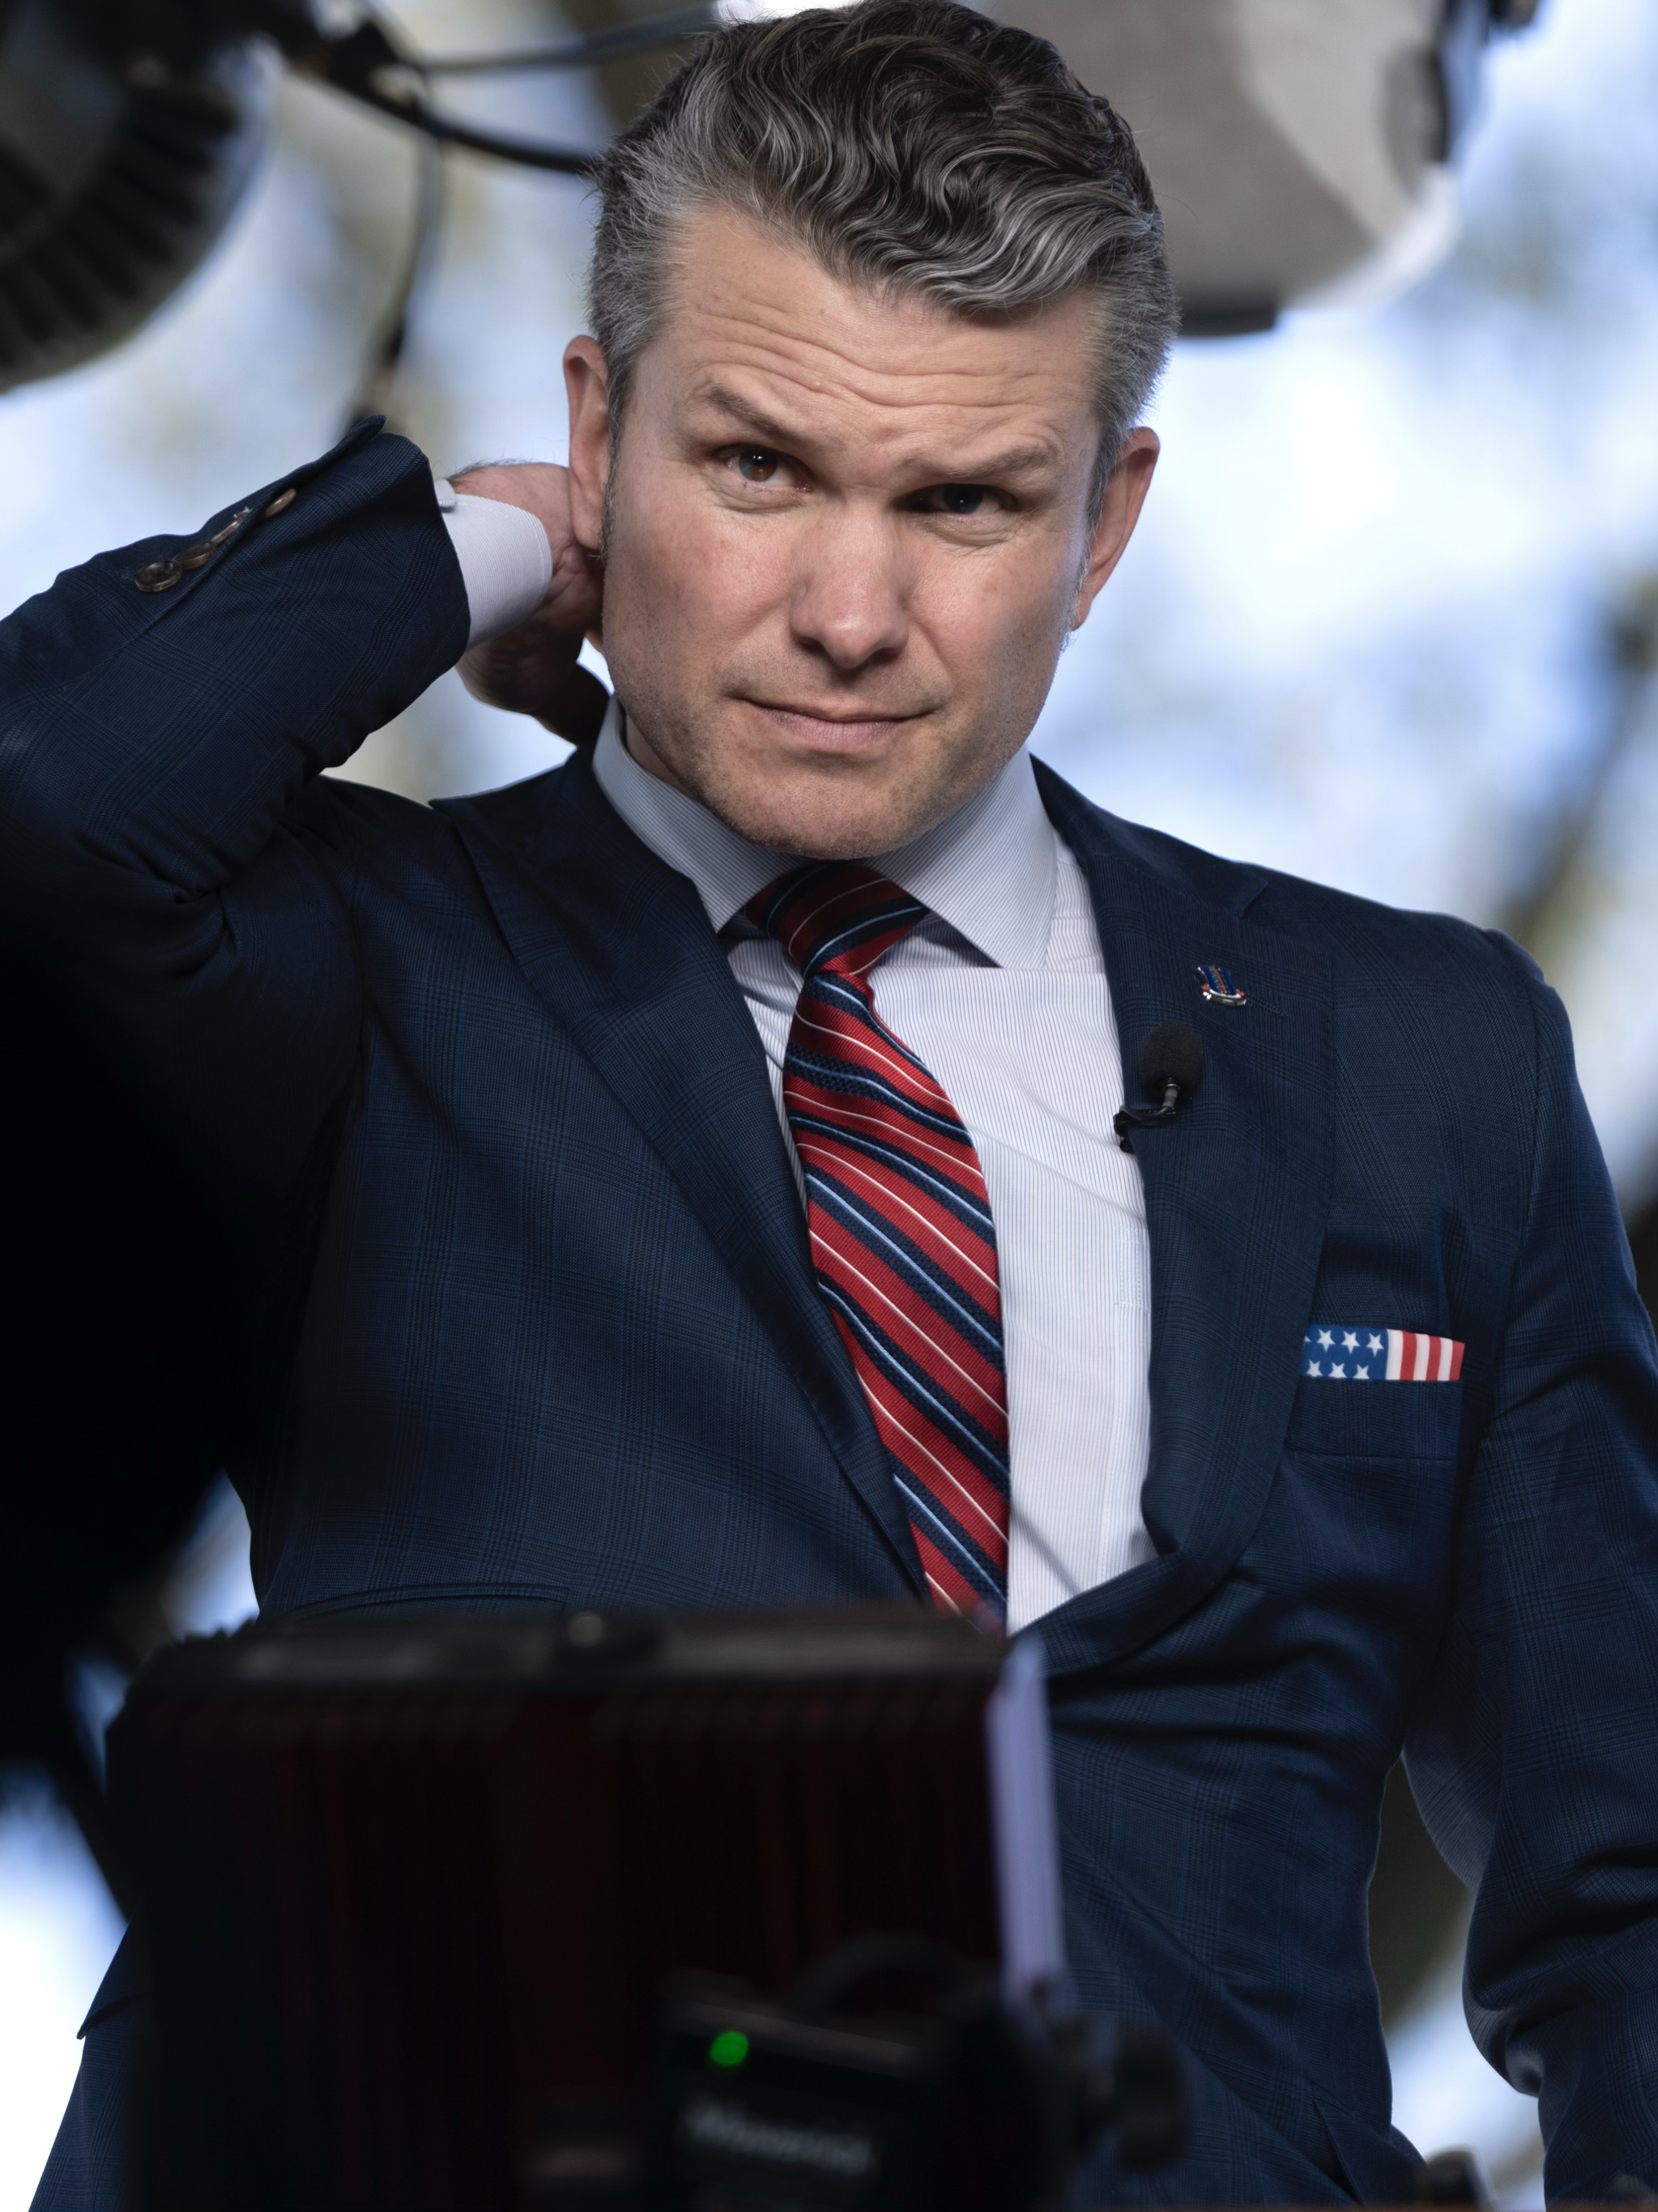
\includegraphics[height=6cm]{./assets/ap_hegseth_cut.png}
                \caption{Pete Hegseth,\\US Secretary of Defense~\cite{coppTrumpOfficialsTexted2025}}
            \end{figure}
        \end{column}
    \end{columns}

    \note{
        \begin{itemize}
            \item wir haben schon viel über Signal gehört
            \item persönliche Motivation: Benutzung von Signal, Signal-Projekt spannend (E2E-Encryption, Open Source)
            
            \item aber ich möchte noch mal ein Beispiel mitbringen, welches hervorhebt, wie relevant dieser Messenger ist
            \item Signal wird selbst von der US-Administration verwendet, um Kriegsgeheimnisse zu teilen
            \item Signal ist nicht sinnvoll knackbar
            \item aktuell braucht es noch menschliche Fehler dafür
            \item Wie macht Signal das?
        \end{itemize}
    }
\end{frame}


\begin{frame}{Einleitung}
    \begin{columns}
        \begin{column}{0.6\textwidth}
            \begin{itemize}
                \item aktuell: X3DH, Double Ratchet etc.
                \pause
                
                \item am Horizont: \alert{Quanten-Computing}
                \begin{itemize}
                    \item[$\Rightarrow$] Lösung von bisher \enquote{unlösbaren} Problemen
                \end{itemize}
                
                \item[$\Rightarrow$] Post-Quanten-Kryptografie
            \end{itemize}
        \end{column}


        \begin{column}{0.3\textwidth}
            \begin{figure}
                \includegraphics[width=\textwidth]{assets/quantum-computing.pdf}
                \caption{Quanten-Computing (Symbolbild)~\cite{zuozuozuozuoQUANTUMCOMPUTINGIcon}}
            \end{figure}
            \vspace{-2em}
        \end{column}
    \end{columns}

    \note<1>{
        \begin{itemize}
            \item Signal versucht uns schon bestmöglich zu schützen, bspw. mit ...
        \end{itemize}
    }
    \note<2>{
        \begin{itemize}
            \item seit mehreren Jahren, leuchtet jedoch noch etwas anderes am Horizont, wodurch Attacken nicht mehr auf menschliche Fehler angewiesen sind
            \item QC $\to$ auf einmal sind bisherige, unknackbare Verschlüsselungstechniken lösbar
            \item Signal auch zukünftig schützen<
            \item dafür brauchen wir PQ-Kryptografie
        \end{itemize}

        \vspace{1em}
        Gliederung:
        $\Rightarrow$ KEM: Alternative zum Public Key Encryption Verfahren
    }
\end{frame}
